\section{Insights into Data Engine Behavior}
\label{sec:insights}
\eat{
In the previous section, we saw that the iterative approach is not scalable as it is expensive to run jobs multiple times. Therefore we set upon an alternative approach of using mathematical models to recommend new settings.} In this section, we study the effect of each parameter on the query cost by performing a set of experiments. These experiments provide key insights that will be the basis to develop a simple mathematical model. All the experiments were run for a Spark engine using the TPC DS dataset (scale 1000) and queries on a 4 node AWS cluster with machine type r3.xlarge.
\eat{
The assumptions made in the iterative approach (Section~\ref{sec:assumptions}) continue to be applicable.} \eat{The experiments focus on a few key parameters, the values are discretized, range of values for each parameter is bounded and the dimensions are independent of each other. }

\begin{figure*}[ht]
\minipage{0.32\textwidth}
  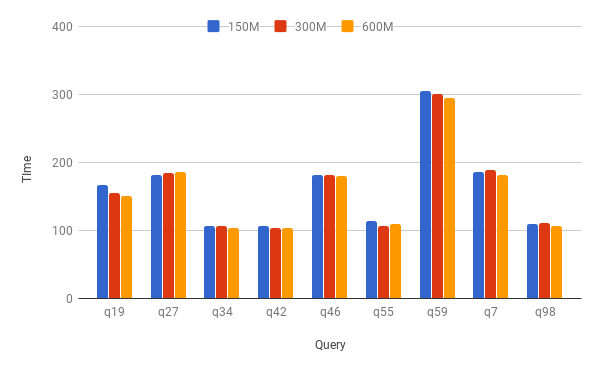
\includegraphics[width=\linewidth]{fig/varysplitsize.png}
  \caption{Varying split size \protect\footnotemark[1]}\label{fig:varysplitsize}
\endminipage\hfill
\minipage{0.32\textwidth}
  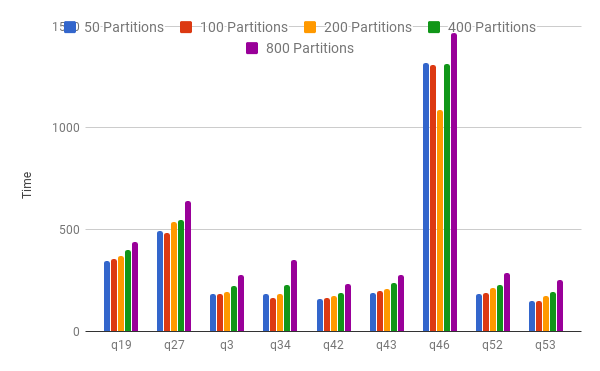
\includegraphics[width=\linewidth]{fig/varyreducers.png}
  \caption{Varying reducer partitions \protect\footnotemark[1]}\label{fig:varyreducers}
\endminipage\hfill
\minipage{0.32\textwidth}%
  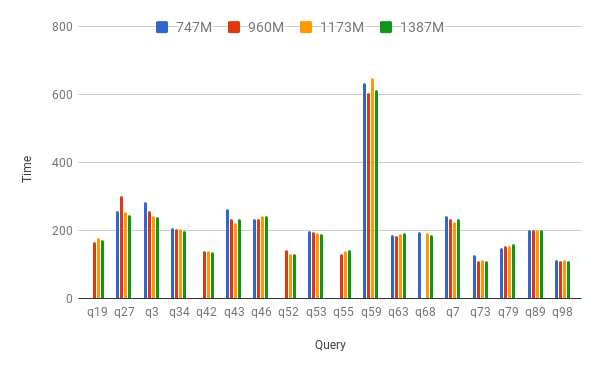
\includegraphics[width=\linewidth]{fig/varymem.png}
  \caption{Varying memory per executor core \protect\footnotemark[1]}\label{fig:varymem}
\endminipage
\eat{\minipage{0.24\textwidth}%
	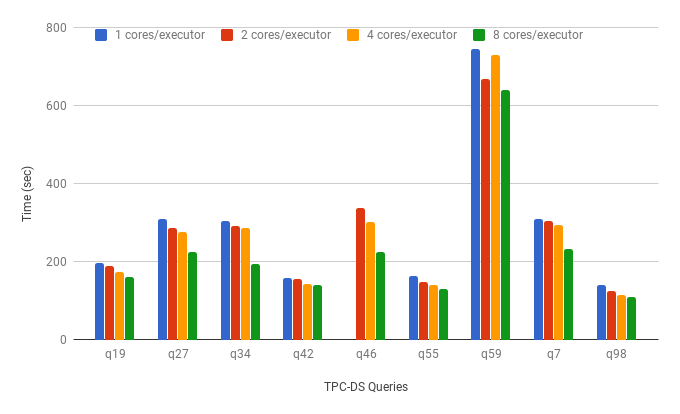
\includegraphics[width=\linewidth]{fig/varycore.png}
	\caption{Varying cores per executor \protect\footnotemark[1]}\label{fig:varycore}
\endminipage}
\end{figure*}

\subsubsection*{Memory and partition size}
We studied the relationship between the container memory and the amount of data processed by the container, i.e. the partition size.  Spark tasks are of two types -- input mapper tasks the process data from the input tables and reducer tasks that process the output from the previous tasks in the pipeline. The splitsize parameters ($split.minsize$ and $split.maxsize$) determine the partitions size for the mapper tasks, whereas the reducer parallelism parameter ($spark.sql.shuffle.partitions$) determines the data processed by each reducer task.
\eat{
 The partition size for the input mapper tasks is referred to as the splitsize and is determined by the parameters %$spark.hadoop.mapreduce.input.fileinputformat.
$split.minsize$ and %$spark.hadoop.mapreduce.input.fileinputformat.
$split.maxsize$. The partition size for the reducer tasks is determined by the reducer parallelism, which is controlled by the parameter $spark.sql.shuffle.partitions$. 
}

Initially, we varied the partition size of the mapper tasks by varying the splitsize from 150 MB to 600 MB while holding all other parameters constant. The memory available to each executor core was 1386 MB, which was sufficient to hold even the largest split of 600 MB, thus avoiding spills. Figure \ref{fig:varysplitsize} shows that the cumulative run time reduces as the splitsize increases. This is because the number of mapper tasks reduces as the splitsize increases. This leads to overall lesser cpu overheads in terms of the number of tasks to be managed. For MR engines, the overhead of starting a JVM for each task can further add to the overhead. Also, reducer tasks down the pipeline have to pull their data from lesser number of mappers, leading to lesser network overheads. Since there are no spills, there is no major negative effect of larger split sizes. However, it can be seen that the overall reduction is not large, with the average being 6.73\%. This is because the total amount of data processed, IO and network traffic is independent of the parallelism; only the overheads vary. 

\eat{
In the first set of experiments, we varied the partition size of the mapper tasks by varying the split parameter while holding all other parameters constant. The splitsize was varied from 150 MB to 600 MB. Based on the container memory, the memory available to each executor core was 1386 MB, which was sufficient to hold even the largest split of 600 MB. Hence, there were no spills in any of the experiments. Figure \ref{fig:varysplitsize} shows the variation of the cumulative run time with the splitsize. Overall, the cumulative run time reduces as the splitsize increases. This is because the number of mapper tasks reduces as the splitsize increases. This leads to overall lesser cpu overheads in terms of the number of tasks to be managed. For MR engines, the overhead of starting a JVM for each task can further add to the overhead. Also, reducer tasks down the pipeline have to pull their data from lesser number of mappers, leading to lesser network overheads. Since there are no spills, there is no major negative effect of larger split sizes. It can be further observed that, though the cumulative time reduces, the overall reduction is not large, with the average being 6.73\%. This is because the total amount of data processed, IO and network traffic is independent of the parallelism, only the overheads vary. 
}
\eat{
\begin{figure}[h]
	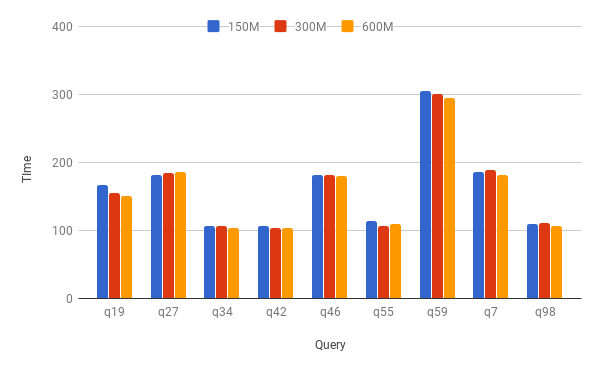
\includegraphics[width=\linewidth]{fig/varysplitsize.png}
	%\vspace*{-15pt}
	\caption{Varying split size \protect\footnotemark[1]}
	\label{fig:varysplitsize}
\end{figure}
}

Next, we varied the partition sizes for the reducer tasks by varying the %$spark.sql. 
reducer parallelism ($shuffle.partitions$) parameter from 50 to 800. The original TPC DS queries have many filters on the input tables, due to which the reducers process very less data and don't contribute much to the cumulative query time. To make this experiment on the reducer parallelism meaningful, we modified the queries to remove all the filters, so that data processed by the reducers becomes significant. Figure~\ref{fig:varyreducers} shows the variations in the cumulative time with the number of partitions. As before, the overall time for the query increases with parallelism, due to increased overheads. The increase is moderate, for e.g., the 16 times increase in parallelism leads to an average slowdown of 47\%. These experiments lead to the next insight:

\eat{
In the second set of experiments, we varied the partition sizes for the reducer tasks by varying the %$spark.sql.
$shuffle.partitions$ parameter from 50 to 800. This varies the number of reducer partitions and correspondingly the amount of data processed by each reducer task. The original TPC DS queries have many filters on the input tables, due to which the mappers process lots of data and the reducers process very less data. The overall time is thus dominated by the mapper tasks. To make this experiment on the reducer parallelism meaningful, we modified the queries to remove all the filters. After this change, the reducer tasks become a significant part of the overall query and changes in reducer times reflect in the overall query times. Figure~\ref{fig:varyreducers} shows the variations in the cumulative time with the number of partitions. As before, the overall time for the query increases with parallelism, due to increased overheads. The increase is moderate, for e.g., the 16 times increase in parallelism leads to an average slowdown of 47\%. These experiments lead to the next insight:
}
\begin{insight}
	\label{insight:parallelism}
	The parallelism of a query can be increased without significant adverse effect to the cumulative time. At the same time, it should not be increased indiscriminately since the increased parallelism leads to increased overheads and increases the overall cumulative time.
\end{insight}
\eat{The increased overheads are due to managing a larger number of tasks and increase in the number of communicating channels. For MR engine, the overhead of starting a JVM for each task can further add to the overhead.}

\eat{
\begin{figure}[h]
	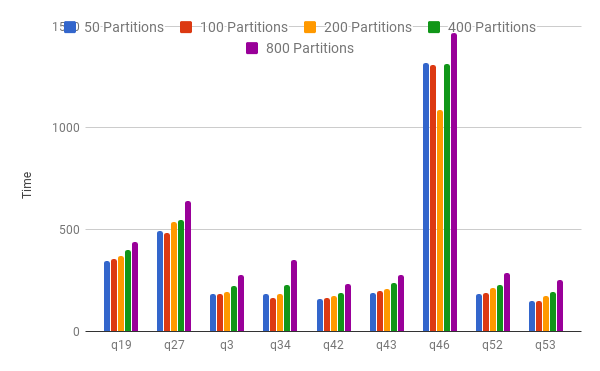
\includegraphics[width=\linewidth]{fig/varyreducers.png}
	%\vspace*{-15pt}
	\caption{Varying reducer partitions \protect\footnotemark[1]}
	\label{fig:varyreducers}
\end{figure}
}

The experiments with reducer parallelism also show the effect of spills on the query time. For example, $q27$, $q34$ and $q46$ cumulative time decreased when parallelism increased from 100 to 200 partitions. Figure~\ref{fig:q46} shows a graph for $q46$, in which the time reduces by almost 30\% when the number of shuffle partitions increases from 100 to 200. This is due to the fact that at 100 partitions, the amount of data processed by the reducer task does not fit in memory and causes a spill. As the number of partitions increases to 200, each partition becomes smaller and fits in memory, thus avoiding a spill. This leads to the following insight:
\begin{insight}
	\label{insight:spill}
	Spills are expensive as each spill leads to an extra write and read of the data. Thus, spills should be avoided at all costs.
\end{insight}
Spills can be avoided by providing adequate memory to each task or by making more fine grained tasks. Since the memory for each container is fixed, we can either reduce the splitsize (for input mapper tasks) or increase the reducer parallelism (for reducer tasks) so that each task processes only data that can fit in its available memory without causing a spill.

\begin{figure}[h]
	\centering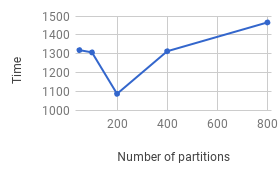
\includegraphics[height=3cm]{fig/q46.png}
	%\vspace*{-15pt}
	\caption{Effect of spill}
	\label{fig:q46}
\end{figure}

\footnotetext[1]{Bars in chart are in the same order as that of legends}

\noindent\subsubsection*{Memory and instance type}
%We saw that the memory of each container should be set according the Memory/vCPU ratio of the machine. 
\eat{Cloud platforms provide a variety of machines which differ in various characteristics such as cpu speed, disk speed, network speed, cpu cores and memory.} Usually, machines with higher memory/cpu core are more expensive for the same CPU type. To evaluate if it worth paying extra for higher memory/cpu core, we \eat{conducted a set of experiments where we} varied the memory available per executor core from 746 MB to 1386 MB in steps of 200 MB, while keeping all other parameters fixed. \eat{The experiments were run on a Spark engine on the TPC DS dataset (scale 1000) and using the TPC DS workload. The average data read by each query was around 20 to 40 GB.} \eat{The experiments were run on a 4 node cluster on AWS with machine type r3.xlarge. We varied the memory per executor core from 746 MB to 1386 MB in steps of 200 MB.} The partition sizes were at the default value of 128 MB, so there is enough memory in all cases to hold the data and there were no spills. Figure~\ref{fig:varymem} shows \eat{the variation in the cumulative time with memory. In most cases, it was observed that} the cumulative cpu time usually decreases as the container memory increases. The decrease is due to lesser pressure on memory and reduced costs of garbage collection. \eat{However, in some cases the time also increases with memory.} However, the variation in cumulative cpu cost with memory was not very significant. Overall the average speedup was 3.5\% and the maximum speed up was 18\% ($q3$). 

\eat{
\begin{figure}[h]
	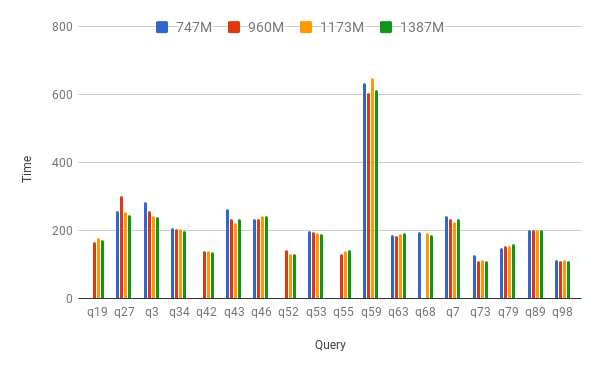
\includegraphics[width=\linewidth]{fig/varymem.png}
	%\vspace*{-15pt}
	\caption{Varying memory per executor core \protect\footnotemark[1]}
	\label{fig:varymem}
\end{figure}
}

\eat{This behavior is due to the way memory is used by the SQL engines.} In SQL engines, memory is mainly used to hold the partition processed by the container (as io.sort.mb in MR and to hold the rdd in Spark). Once there is enough memory to hold the partition in memory (thus avoiding spills), any increase beyond that does not have any additional benefit.
As long as tasks do not spill, the total work done in terms of IO, CPU and network traffic is independent of the available memory and the parallelism factor of the tasks. This leads to the following insight:
\begin{insight}
	\label{insight:mem}
	For a query, the memory per task can be decreased safely without performance degradation by correspondingly decreasing the partition size (increasing parallelism) if needed to avoid spills.
\end{insight}
This implies that 
if a job can be tuned to avoid spills on a cheaper instance with same compute but lesser memory than original instance, then it is generally a good idea to move to cheaper instance for saving cost without any performance degradation.

\subsubsection*{Cores per executor}
For Spark engines, there is an additional parameter of cores per executor. Given a certain number of cores per machine, we have a choice of either running many executors with fewer cores per executor (thin executors), or fewer executors with more cores per executor (fat executors). We varied $spark.executor.cores$ from 1 to 8 and correspondingly varying $spark.executor.memory$ from 1152MB to 11094MB, thus keeping memory per core constant.
\eat{We studied the effect of various choices by varying the $spark.executor.cores$ from 1 to 8 and correspondingly varying $spark.executor.memory$ from 1152MB to 11094MB. The memory per executor core is the same in all cases. Figure~\ref{fig:varycore} shows the variation in the cumulative time with number of cores.} It can be observed from Figure~\ref{fig:varycore} that fat executors generally provide better performance (upto 25\%). \eat{On an average, there was a 25\% speedup on using 8 cores per executor compared to 1 core per executor.} Fatter executors perform better because of several reasons such as  better memory utilization across cores in a executor, reduced number of replicas of broadcast tables and lesser overheads due to more tasks running in the same executor process. This leads to the following insight specific to Spark engines:
\begin{insight}
	\label{insight:executorcore}
	Use a single fat executor for each node that uses up all the cores on the node rather many thin executors.
\end{insight}

\begin{figure}[h]
	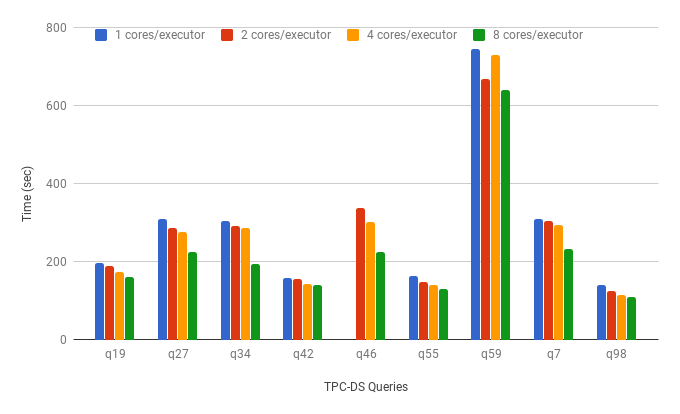
\includegraphics[width=\linewidth]{fig/varycore.png}
	%\vspace*{-15pt}
	\caption{Varying cores per executor \protect\footnotemark[1]}
	\label{fig:varycore}
\end{figure}

\footnotetext[1]{Bars in chart are in the same order as that of legends}
